\documentclass[11pt]{article}
\usepackage[margin=1in]{geometry}
\usepackage{booktabs}
\usepackage{graphicx}
\usepackage{microtype}
\usepackage[hidelinks]{hyperref}

\newcommand{\NPapers}{3,073,288}
\newcommand{\NCitations}{176,934,085}
\newcommand{\NResolved}{70,634,716}
\newcommand{\NEdges}{36,688,723}
\newcommand{\ResPct}{39.9\%}


\title{\vspace{-2em}\textbf{Experiment 03 — Citation-graph structure}}
\author{arxivkg · preprocessing · phase 3/4 (graph)}
\date{}

\begin{document}
\maketitle
\vspace{-2em}

\section*{What we did}
Characterize the intent-typed citation graph --- the substrate phase-6 retrieves over --- read from
the single Postgres+pgvector store: scale, in/out-degree distributions, per-edge intent/polarity
typing, citation growth, and the top-cited papers. Pure SQL + figures, no LLM; heavy aggregations
cached to \texttt{cache/summary.json}.

\section*{Global counts}
\begin{center}\begin{tabular}{lr}
\toprule
metric & value \\
\midrule
papers (nodes) & 3,073,288 \\
citation occurrences & 176,934,085 \\
resolved occurrences & 70,634,716 \\
distinct edges & 36,688,723 \\
\bottomrule
\end{tabular}
\end{center}
\NPapers{} papers, \NCitations{} citation occurrences, \NResolved{} resolved (\ResPct), \NEdges{}
distinct edges.

\section*{Degree distributions}
Both in- and out-degree are heavy-tailed (near scale-free): a few papers accrue enormous in-degree
while most are cited rarely --- the hub structure phase-6's pool induction avoids by ranking
\emph{within} an on-topic pool rather than expanding from hubs.

\begin{center}
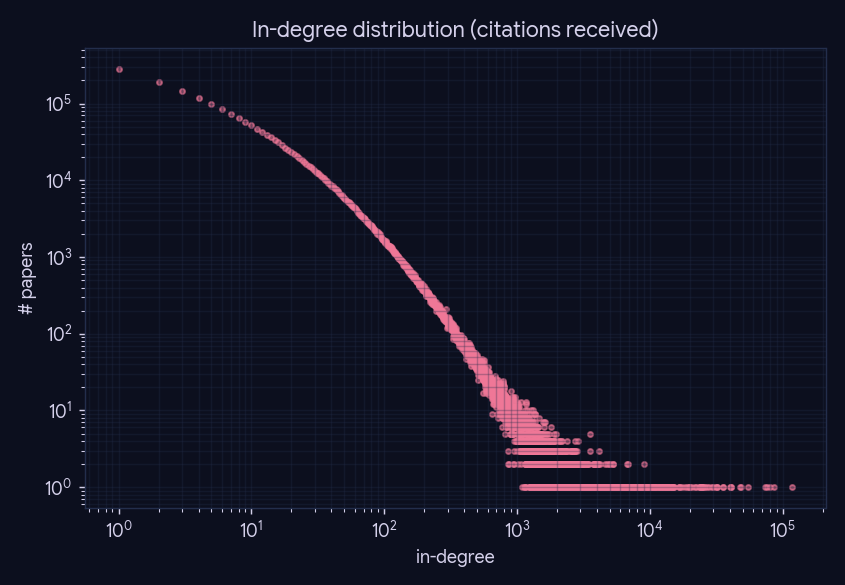
\includegraphics[width=0.49\textwidth]{../results/indegree_loglog.png}
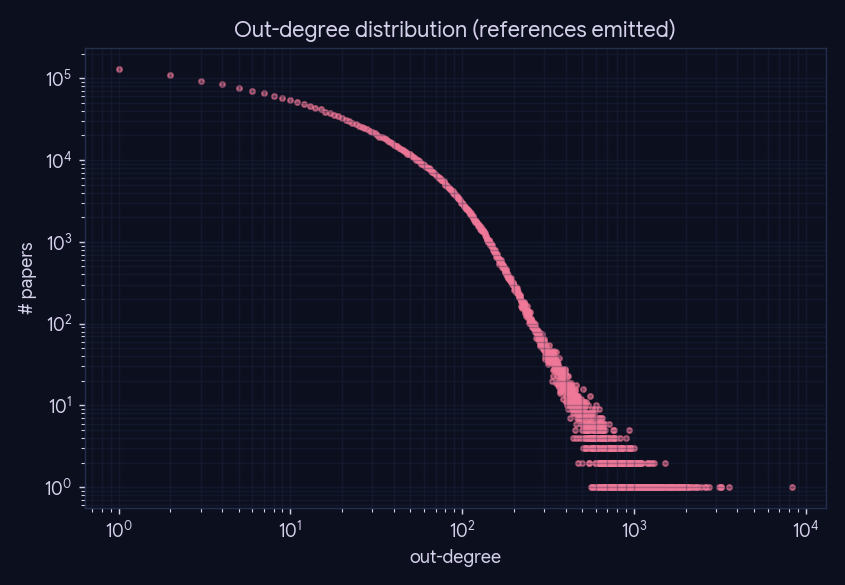
\includegraphics[width=0.49\textwidth]{../results/outdegree_loglog.png}
\end{center}

\section*{Edge typing (the differentiator)}
Every resolved edge carries an intent + polarity. The mix is dominated by
\texttt{background}/\texttt{uses}; the rare relational intents feed phase-6's tensions surfacing.

\begin{center}
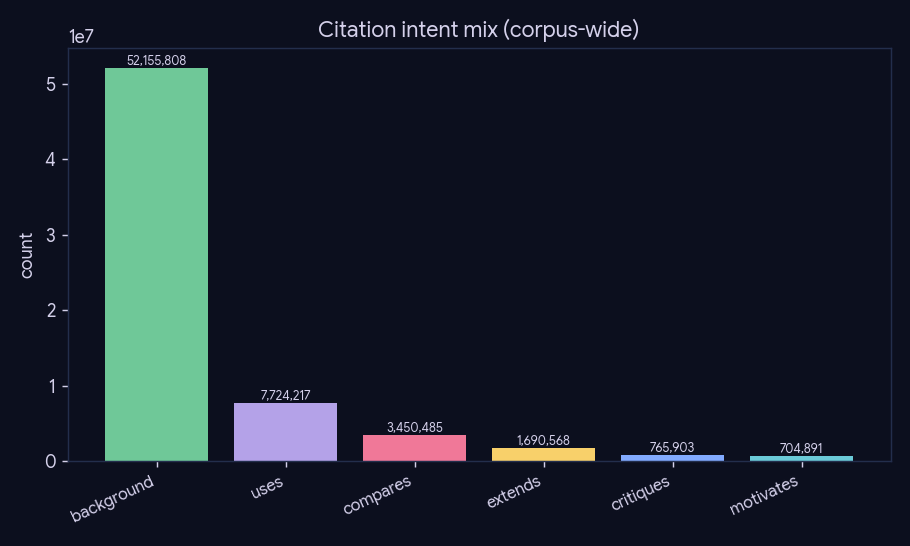
\includegraphics[width=0.49\textwidth]{../results/intent_mix.png}
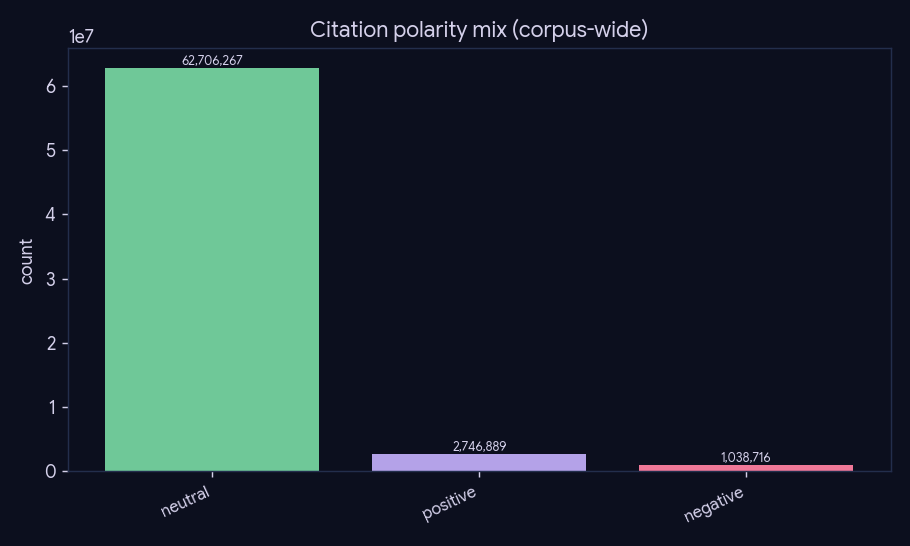
\includegraphics[width=0.49\textwidth]{../results/polarity_mix.png}
\end{center}

\section*{Citation activity over time}
\begin{center}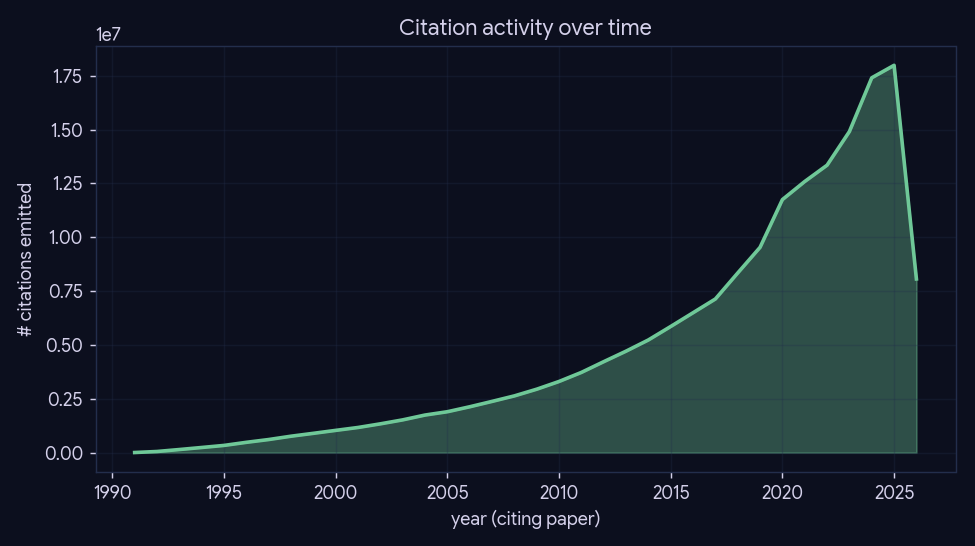
\includegraphics[width=0.7\textwidth]{../results/per_year.png}\end{center}

\section*{Conclusion}
A \textbf{36.7M-distinct-edge}, intent-typed, near-scale-free citation graph over \textbf{3.07M}
papers, whose in-degree ranking recovers the field's landmark papers (ResNet, BERT, Transformer,
CLIP, \ldots --- full table in \texttt{results/metrics.md}). The heavy-tailed hubs motivate the
"induce within a topical pool" design, and per-edge typing is what distinguishes this substrate from
a plain citation graph. In-degree is within-corpus (arXiv$\rightarrow$arXiv resolved only).

\end{document}
